\documentclass[a4paper, 12pt]{article}
\usepackage{a4wide}
\usepackage{acronym}
\usepackage{graphicx}
\usepackage[title,titletoc,toc]{appendix}


\begin{document}

\begin{center}
{\LARGE\bf Travelling Thief Problem}\\
\vspace{0.5cm}
{\Large\bf Evolutionary Computation}\\
\vspace{1cm}
Prepared by William Reid, Matthew Hart, Samantha Peachey \& Alec Bellati\\
\vspace{1cm}
School of Computer Science,\\
The University of Adelaide\\
\vspace{1cm}
\today
\end{center}

\section*{Exercise 3}
This exercise focusses on the modification of the tour that our thief takes, based upon a given set of items that he wants to steal. These items are supplied in a text file that is read in. Since this problem revolves around solving the traditional travelling salesman problem (with a few restrictions), evolutionary approaches should yield good results within the required time-frame. 

\section{Algorithm}
This algorithm performs four fundamental steps:

\begin{enumerate}
\item Seed the knapsack with items using various methods
\item Seed a random tour, taking into account the packing plan
\item Evaluate solution
\item Mutate tour
	\begin{itemize}
		\item A subset of the tour is selected to be scrambled. 
		\item This subset is randomly shuffed around, checking to ensure that the order specified by the packing plan is not disrupted. 
	\end{itemize}

\end{enumerate}
Steps 3 and 4 are then repeated, generating new individuals and selecting the fittest individual to continue generating. Scrambling was chosen as the mutator of choice as it was found to be quite powerful during assignment 1. 

\newpage

\subsection{Profit Evaluation}
To evaluate the profit of the solution at each step, the evaluate function from the TTPInstance class was used. This ensures that the calculated profit uses the correct formulas and also reduces the code base. Research was done into faster evaluation methods and while it is possible to create a simpler (but less accurate) evaluation technique, the gains were not significant enough for the implementation of a new method.

\subsection{Useability on Problem Types}

The primary bonus in the choice of this algorithm is it ensures it will behave in similar ways, no matter how the problem is presented. Whether it be strongly bounded, uncorrelated, single item per city, multiple items per city or thousands of cities - the algorithm will be consistent. 

\section{Testing, Additional Methods and Results}

Some different methods were considered to try and better the result of the solution. This included different methods of seeding the original knapsack, and additional methods for modifying the TSP (such as swapping or inversion of cities within the tour). While these methods served as useful tests and concepts, they did not prove profitable within the algorithm. \\

The results of this algorithm were not as ideal as other approaches considered. This problem can be reduced to finding the shortest path through a graph, with required checkpoints at given stages. Given the limitations in regards to the items that need to be collected, this simply becomes a matter of minimising the rent paid and there are not many other variables that can influence this. \\

\begin{figure}[h]
\centering
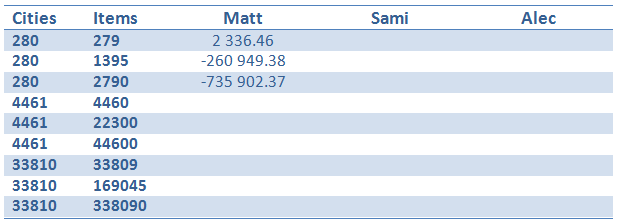
\includegraphics[width=80mm]{AlgorithmResults.png}
\end{figure}

Using the cost first approach to generating the knapsack, negative values were consistently produced. This approach was run using n = 10,000 generations (this was found to be the optimal number of generations in assignment 1), and the improvement over such a large number of generations was minimal. \\

The same can be said of the random knapsack generation, however over significantly smaller generation sizes (n = 10, n = 100), this approach saw a significantly better improvement from the initial starting position. The random knapsack generation approach also works much better than the cost first approach for both the bounded strong correlated and uncorrelated but similar weights problems, yet for the uncorrelated, dissimilar weights problems, the random knapsack seed was consistently worse. \\

It can be seen that the initial knapsack packing has a significant impact upon the performance of the travelling thief, and if this is suboptimal, there is not much that can be done to rectify the situation. It is also quite possible that there is a problem with my implementation, given the extremely negative figures, or in some instances, extremely high figures. 

\end{document}